\documentclass[conference]{IEEEtran}
\IEEEoverridecommandlockouts
\usepackage{amsmath,amssymb,amsfonts}
\usepackage{algorithmic}
\usepackage{graphicx}
\usepackage{textcomp}
\usepackage{xcolor}
\usepackage{booktabs}

\def\BibTeX{{\rm B\kern-.05em{\sc i\kern-.025em b}\kern-.08em
    T\kern-.1667em\lower.7ex\hbox{E}\kern-.125emX}}
\begin{document}

\title{Performance Metrics for Evaluating Internet Speed Test in a Symmetric Broadband\\
}

\author{\IEEEauthorblockN{1\textsuperscript{rd} Nathan Joshua Sucgang}
\IEEEauthorblockA{\textit{Department of Electronics, Computer, and Communications Engineering} \\
\textit{Ateneo De Manila University}\\
Quezon City, Philippines \\
nathan.sucgang@student.ateneo.edu}
\and
\IEEEauthorblockN{2\textsuperscript{rd} Geoffrey Miguel Guy}
\IEEEauthorblockA{\textit{Department of Electronics, Computer, and Communications Engineering} \\
\textit{Ateneo De Manila University}\\
Quezon City, Philippines \\
geoffrey.guy@student.ateneo.edu}
}

\maketitle

\begin{abstract}
	The internet has become more than a routine of everyone's life; 
    it has become a necessity. This paper aims to use statistics to identify the different factors that affect many aspects of the internet such as its download speed, upload speed, and ping. 
    The research looks at various factors for the causes and changes in the internet's performance such as the location of the household receiving the signal for their internet. 
    With this research information, the researchers of the paper intend to determine the internet's performance metrics from a particular internet service provider (PLDT) in order to leave the issue in the hands of organizations who have the capacity to combat these same hindrances. 
    This data could also further improve the internet performance for the population, consequently improving a conventional part of urban societal life.
\end{abstract}

\begin{IEEEkeywords}
ping, download speed, upload speed, internet
\end{IEEEkeywords}

\section{RANDOM VARIABLES AND SOURCES OF DATA}
\begin{enumerate}
    \item[1.]
    \textbf{Location}:
    The location of the closest test server where the test is being conducted.

    \textbf{Source}: Data gathered from the Ookla Speedtest using Raspberry Pi 4. 
    \item[2.]    
    \textbf{Download Speed}: 
    How fast you can receive data from the internet to your device (measured in Mbps).

    \textbf{Source}: Data gathered from the Ookla Speedtest using Raspberry Pi 4. 
    \item[3.]
    \textbf{Upload Speed}:
    How fast you can send data from your device to the internet (measured in Mbps). 
    
    \textbf{Source}: Data gathered from the Ookla Speedtest using Raspberry Pi 4. 
    \item[4.]
    \textbf{Ping}: 
    A type of latency measurement that sends a small packet of data from your device to a server and back (measured in ms).

    \textbf{Source}: Data gathered from the Ookla Speedtest using Raspberry Pi 4. 
    \item[5.] 
    \textbf{Jitter}: 
    Variation in latency over time (measured in ms).

    \textbf{Source}: Data gathered from the Ookla Speedtest using Raspberry Pi 4. 
\end{enumerate}

\section{NORMALITY OF DATA}
\begin{enumerate}
    \item[1.]    
    \textbf{Download Speed}: 
    \begin{enumerate}
        \item \textbf{Test}: Kolmogorov-Smirnov Test
        \item \textbf{Result}: D = 0.2535, p-value = 0 (not normal)
    \end{enumerate}

    \item[2.]
    \textbf{Upload Speed}:
    \begin{enumerate}
        \item \textbf{Test}: Kolmogorov-Smirnov Test
        \item \textbf{Result}: D = 0.1422, p-value = 0 (not normal)
    \end{enumerate}

    \item[3.]
    \textbf{Ping}:
    \begin{enumerate}
        \item \textbf{Test}: Kolmogorov-Smirnov Test
        \item \textbf{Result}: D = 0.3123, p-value = 0 (not normal)
    \end{enumerate}
\end{enumerate}

\section{METHODOLOGY}
\begin{figure}[!htbp]
\centerline{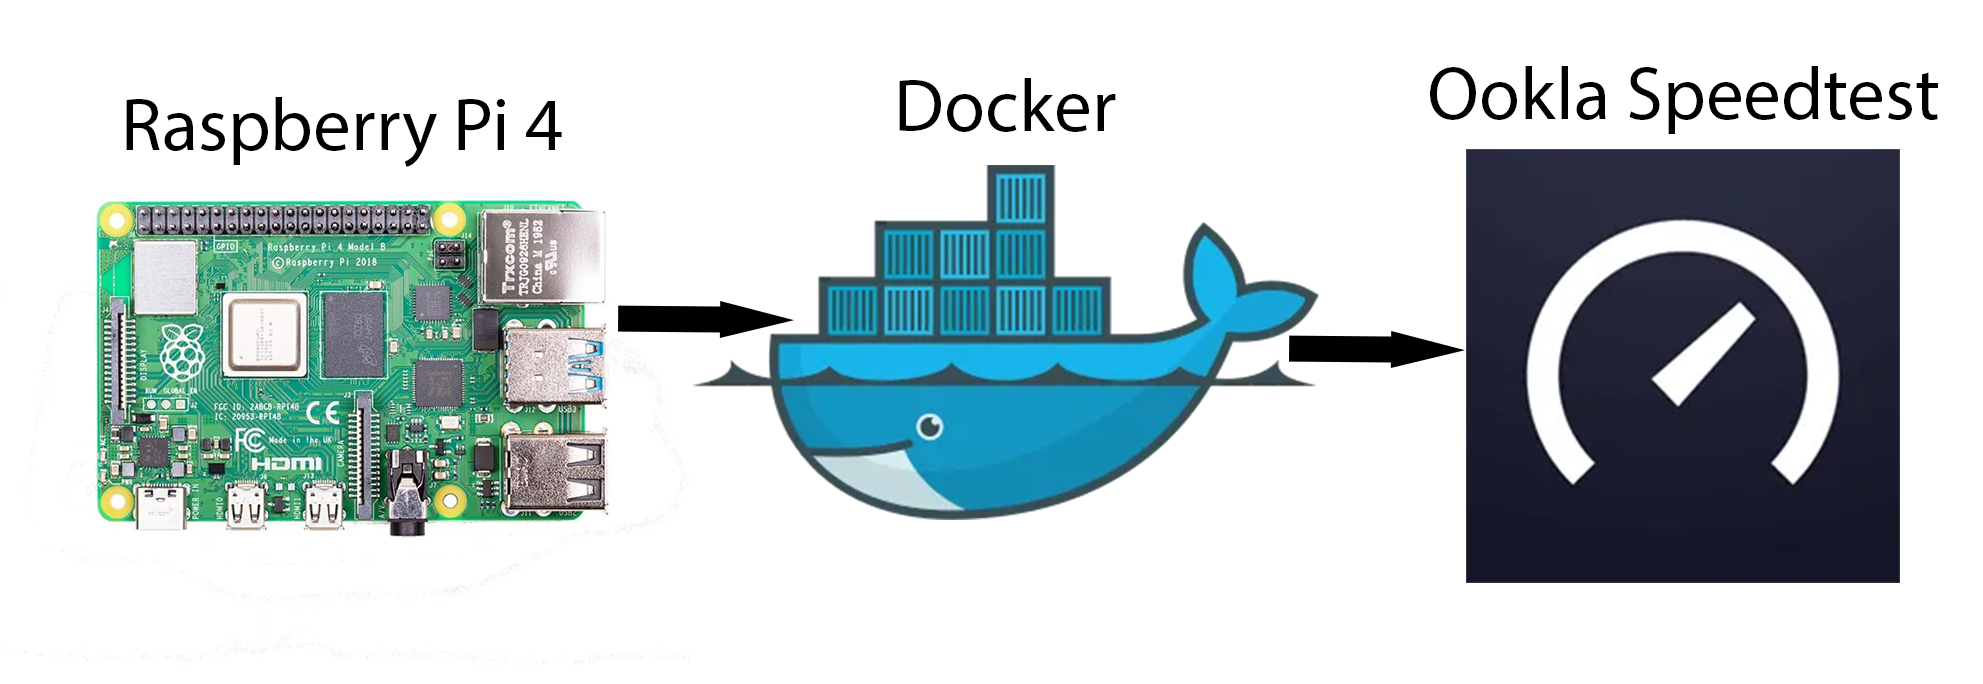
\includegraphics[width=8cm,height=6cm,keepaspectratio]{Figures/Picture0.png}}
\caption{A scenario in evaluating internet speed test.}
\label{fig1}
\end{figure}
As shown in Fig. 1. The Methodology involve collecting data from the Ookla Speedtest using Raspberry Pi 4.
The experiment was conducted from June 19 to July 10, 2024 amounting to 2149 data points. The dataset was cleaned by removing any test from any error that came with misconfigured network.
Statistical analyses, including box plot, class interval, time series graph, was used to examined the relationship between download speed, upload speed, ping and jitter.
MS Excel and Stat Kingdom was used to analyze the data. The statistical analysis was done to determine the factors that affect the internet speed test.

\section{LITERATURE REVIEW}

The internet operates by sending network access from an Internet Service Provider (ISP) from their Optic Line Terminal (OLT), which sends information through a line to an Optic Network Terminal (ONT), which is then given to customers via signal. In Thailand, Boonsongsrikul et al. [3] presented data that clearly shows how the speed of an internet network could exceed its advertised internet speed plan. However, this research gave a warning about the Optical Time Domain Reflectometer (OPTDR), which was the device that was used in evaluating the internet performance metrics during the experiment, that it is not exactly a device used for evaluating internet performance everyday. Furthermore, Sharma et al. [9] showed that changing an ISP will not make much of a difference if a client uses bottleneck WiFi, which is a concept that says the speed of WiFi that a gadget receives is different from the internet's access connection.

On the other hand, Bebortta and Das [2] showed that individuals should pay attention to the type of internet that they are using such as: broadband, cellular data, and etc. For instance, in their methodology they used 4G-LTE, or cellular data internet, to evaluate that the best performing online meeting platform is Microsoft Teams. On the other hand, Deng et al. [4] examined the differences in broadband ISP's speed performance, then concluded that the ISP does not really affect the broadband's performance through statistical tests such as the spearman rho. Likewise, Saengsai et al. [8] evaluated the performance of the broadband internet around the provinces in Thailand with their very own broadband internet speed dashboard, which concluded that ISP's should improve their upload speed.

Individuals also use different software programs to test internet speed, which may influence the measurement of their internet's performance metrics. On their official website, Speedtest [6] mentioned that they use the TCP Test Components and HTTP Legacy Fallback Testing to evaluate internet speed. The information gathering methods from speedtest simply measure how a unit of data (ping) and a chunk of data (download and upload) move around a computer and the network that is connected to this same computer. Similarly, a Bauer et al. [1] stated that Ookla usually results in higher measured data rates compared to other internet speed testing softwares, while also discussing how Ookla gathers its data by filtering 10\% of their fastest data and 30\% of their slowest data.

Research data also encompassed the topic of people's understanding of the internet. A Hasan and Woo [10] indicated that older adults, particularly those in America, evaluate the quality of their internet by relying on the performance of the internet on their devices and their “tech savvy” relatives. This information suggests that some old adult Americans do not understand internet 'jargon.' However, Ikhsan et al. [5] showed that some people, whose mean monthly income is 4 to 15 million rupiahs, rely on network quality, customer service, information quality, security, and privacy for the evaluation of their internet. ISP's monitor this kind of information to maintain customer loyalty.

Futhermore, in the Philippines, the department of Information and Communications Technology (DICT) [7] released a proposal to provide free internet access for public spaces. This internet is meant to be provided to public universities, government offices, and some open areas. However, the minimum goal internet download speed in the proposal is only 2 mbps. This paper shows how the Philippines understands the importance of providing internet to the public and an internet's performance metrics to reach their aim to provide free accessible internet for the Filipino people.

\section{HYPOTHESIS}
\textbf{Hypothesis 1:} The internet speed will not exceed the customer's plan.
\begin{itemize}
    \item \textbf{Alternative Hypothesis:} The internet speed will exceed the customer's plan.
    \item \textbf{Research Gap:} There is no set parameter for the customer to consistently and continuously monitor their internet to determine the instances whether the internet could exceed or fall short from the customer's plan or not. Additionally, there are no definite measures to determine whether the provider of the internet gives their customer the actual or precise speed for their agreed internet plan.
\end{itemize}

\section{PRELIMINARY FINDINGS}
\begin{table}[htbp]
    \centering
    \caption{Performance Metrics}
    \begin{tabular}{lcccc}
        \textbf{Metric} & \textbf{Download} & \textbf{Upload} & \textbf{Ping} & \textbf{Ping Jitter} \\
        Minimum Speed & 424,178,432.00 & 349,885,080.00 & 0.60 & 0.01 \\
        Maximum Speed & 632,378,064.00 & 937,171,528.00 & 23.43 & 6.80 \\
        Range & 208,199,632.00 & 587,286,448.00 & 22.83 & 6.80 \\
        Average Speed & 613,848,923.58 & 755,099,199.14 & 1.18 & 0.22 \\
        Standard Deviation & 16,953,616.30 & 126,111,638.94 & 0.62 & 0.34 \\
        First Quartile & 612,557,732.00 & 640,717,752.00 & 0.97 & 0.09 \\
        Second Quartile & 615,269,336.00 & 796,300,520.00 & 1.00 & 0.15 \\
        Third Quartile & 621,965,420.00 & 863,336,088.00 & 1.38 & 0.23 \\
        Interquartile Range & 9,407,688.00 & 222,618,336.00 & 0.41 & 0.14 \\
        Percent Error & 2.31\% & 25.85\% & 17.94\% & N/A \\
    \end{tabular}
    \label{tab:performance}
\end{table}
We can see the graphical representation, for TABLE 1 in Fig. 1 and Fig. 2.
In the analysis of the data, we used logarithm transform to reduce the variability of data, given that the data set is skewed.
We used one-sample t-test because it determines if the mean of a single sample is significantly different from a known population mean.
For the download speed, we have signifance level of 0.01 and the expected mean of 600000, with the outliers included. 
The result is the difference between the sample average and the expected average is big enough to be statistically significant. 
In other words, we can reject the null hypothesis for the download speed.
For the upload speed, we have signifance level of 0.01 and the expected mean of 600000, with the outliers included. 
The result is the difference between the sample average and the expected average is big enough to be statistically significant. 
In other words, we can reject the null hypothesis for the upload speed.
For the ping, we have signifance level of 0.01 and the expected mean of 1, with the outliers included. 
The result is the difference between the sample average and the expected average is big enough to be statistically significant. 
In other words, we can reject the null hypothesis for the ping.
Futhermore, we can see how the internet speed change through time and how ping change through time in the Fig. 7 and Fig. 8.

\begin{figure}[!htbp]
    \centerline{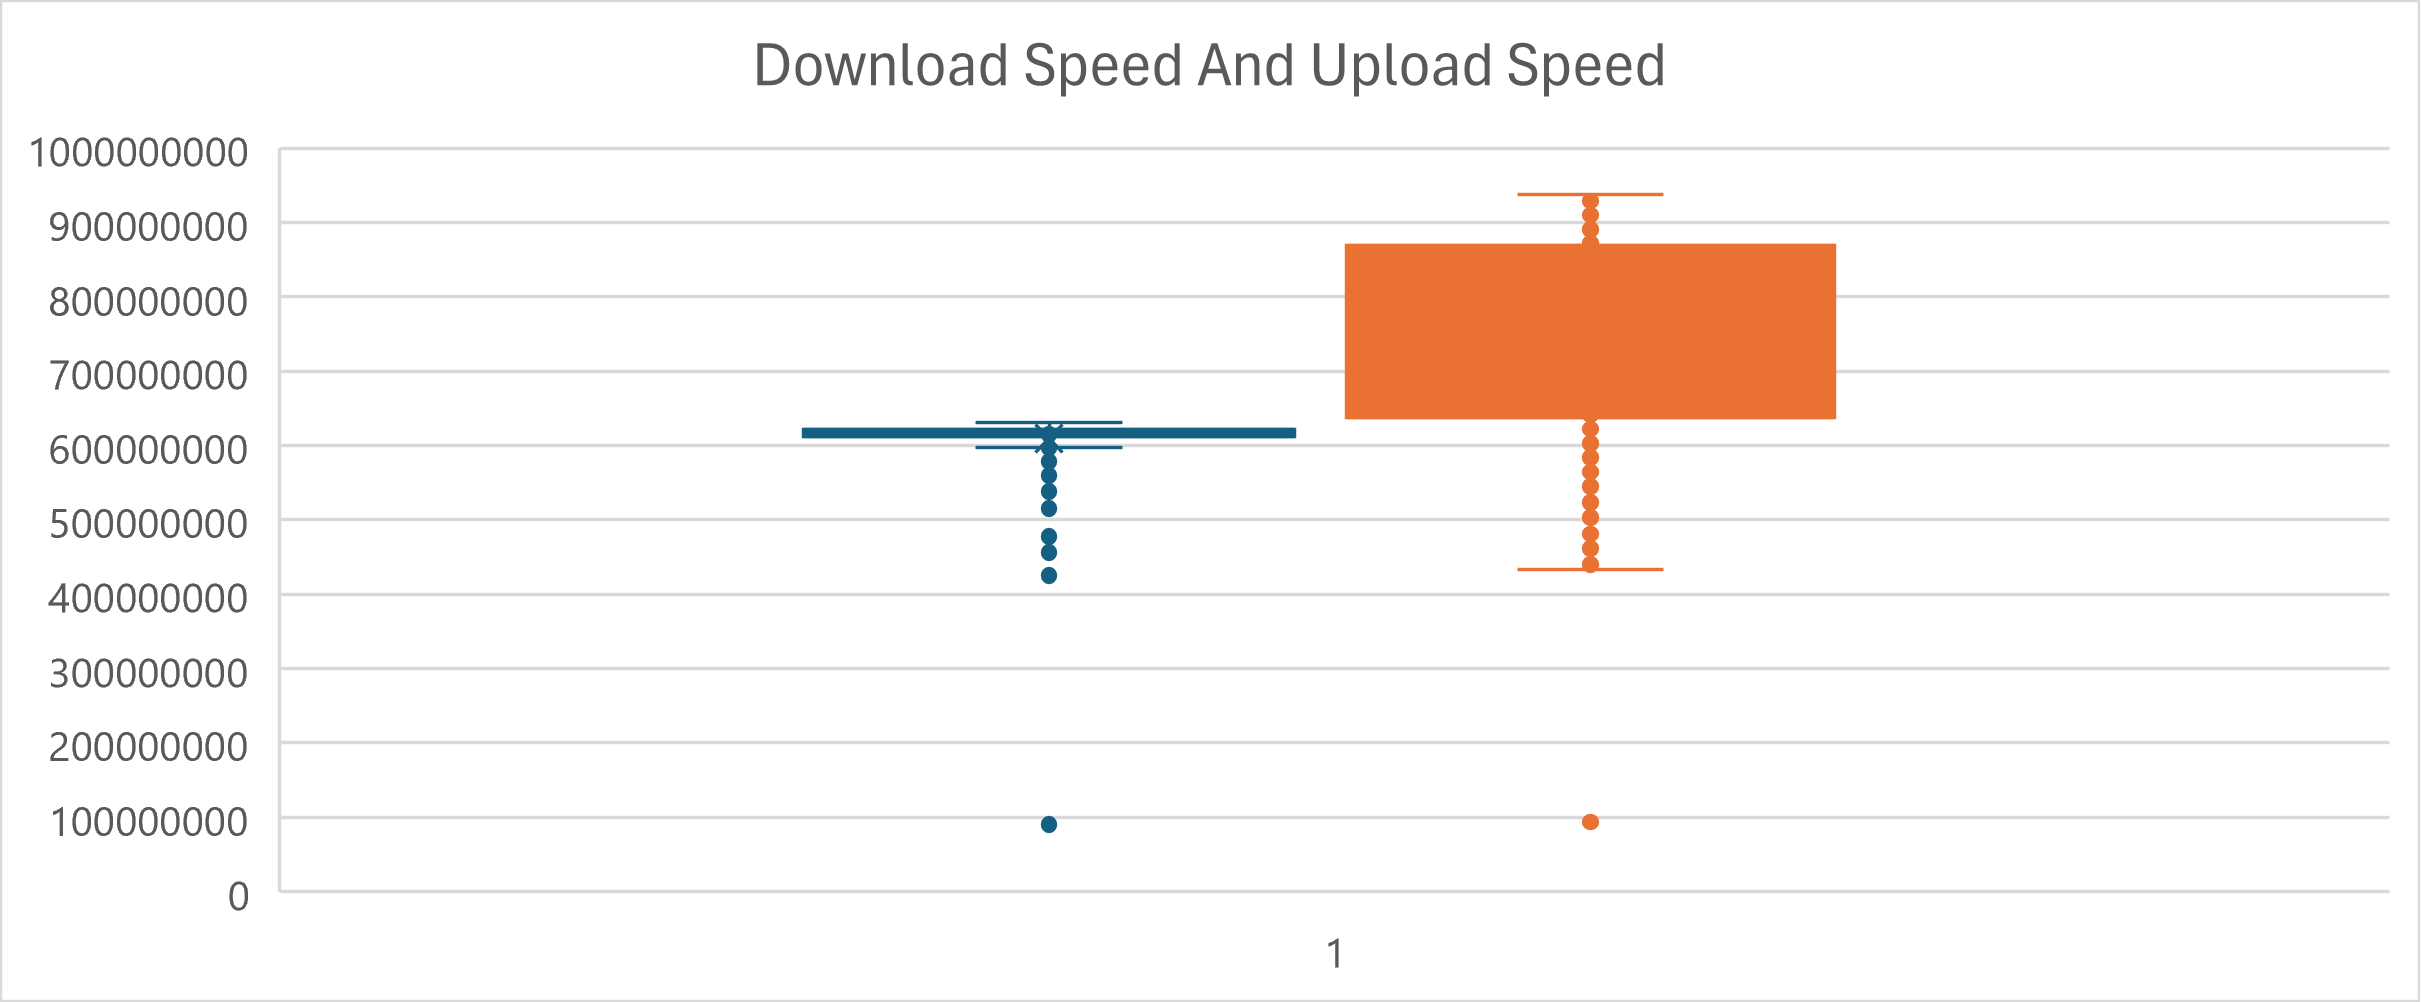
\includegraphics[width=8cm,height=6cm,keepaspectratio]{Figures/Picture1.png}}
    \caption{Box Plot for Internet Speed.}
    \label{fig2}
\end{figure}

\begin{figure}[!htbp]
    \centerline{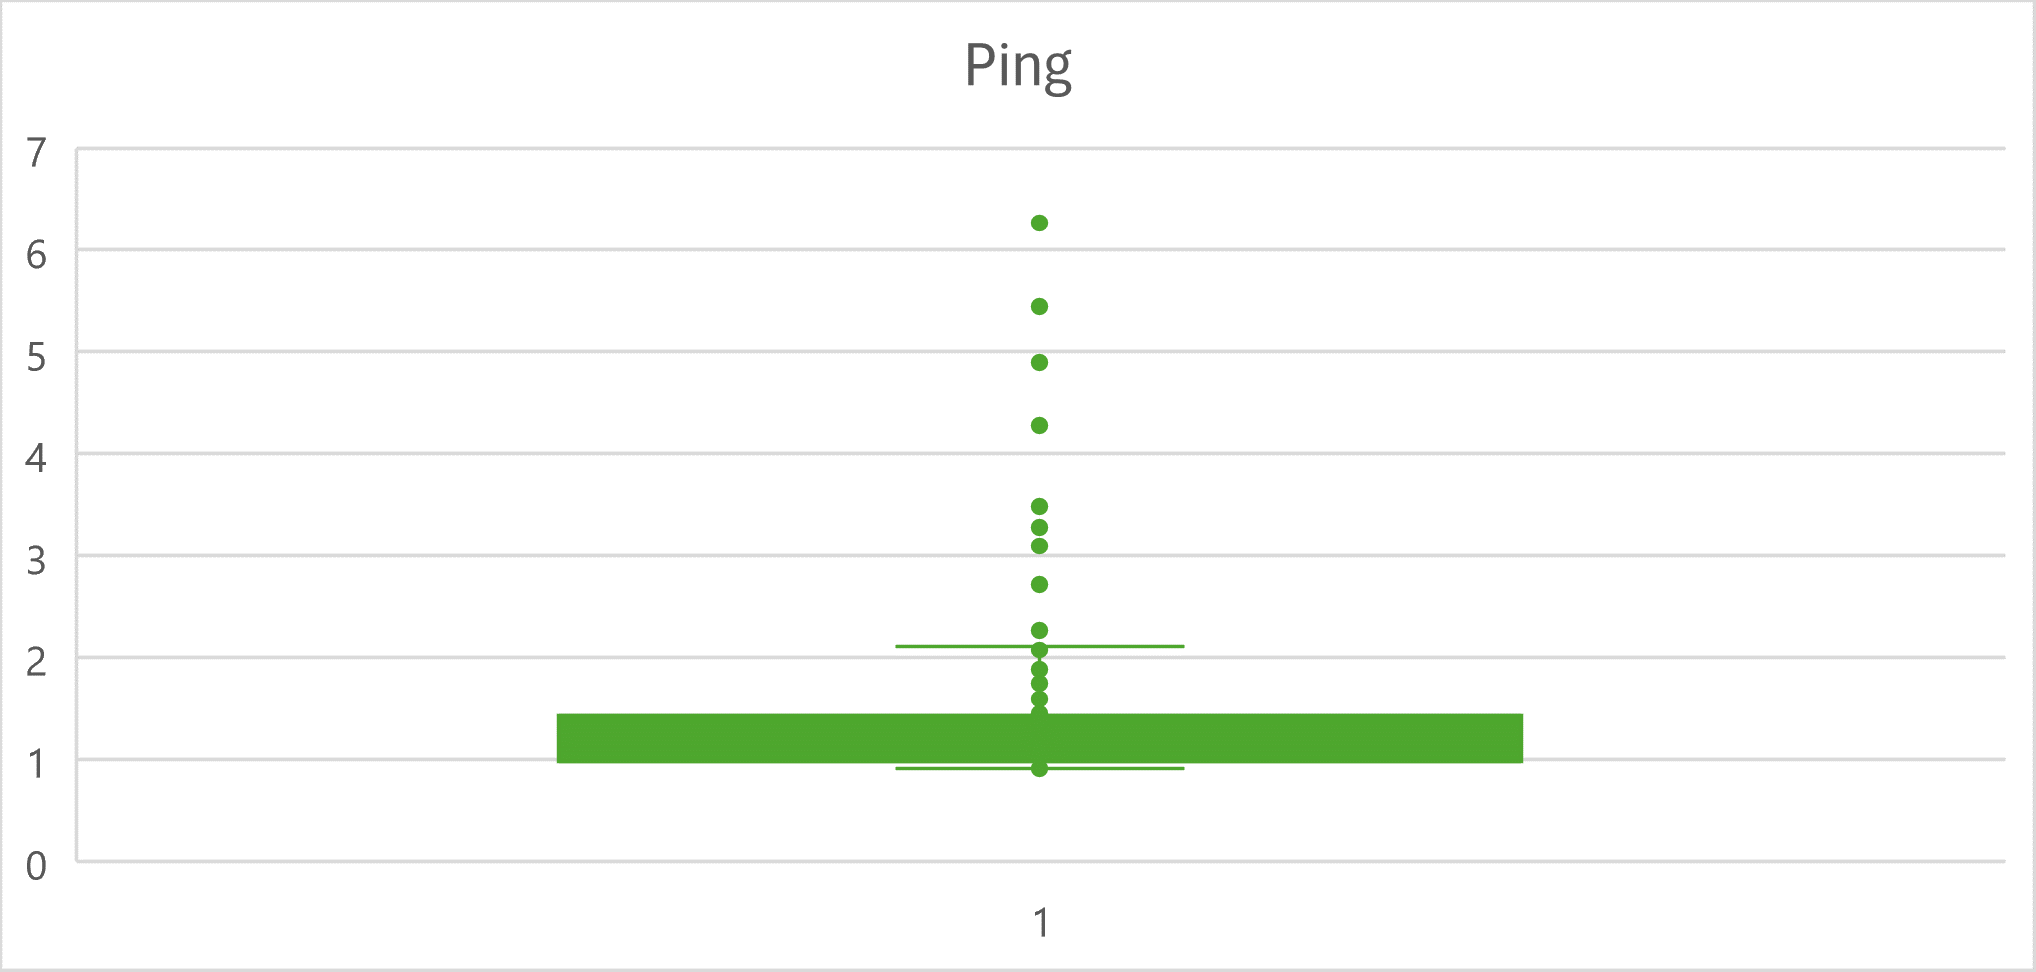
\includegraphics[width=8cm,height=6cm,keepaspectratio]{Figures/Picture2.png}}
    \caption{Box Plot for Ping.}
    \label{fig3}
\end{figure}

\begin{figure}[!htbp]
    \centerline{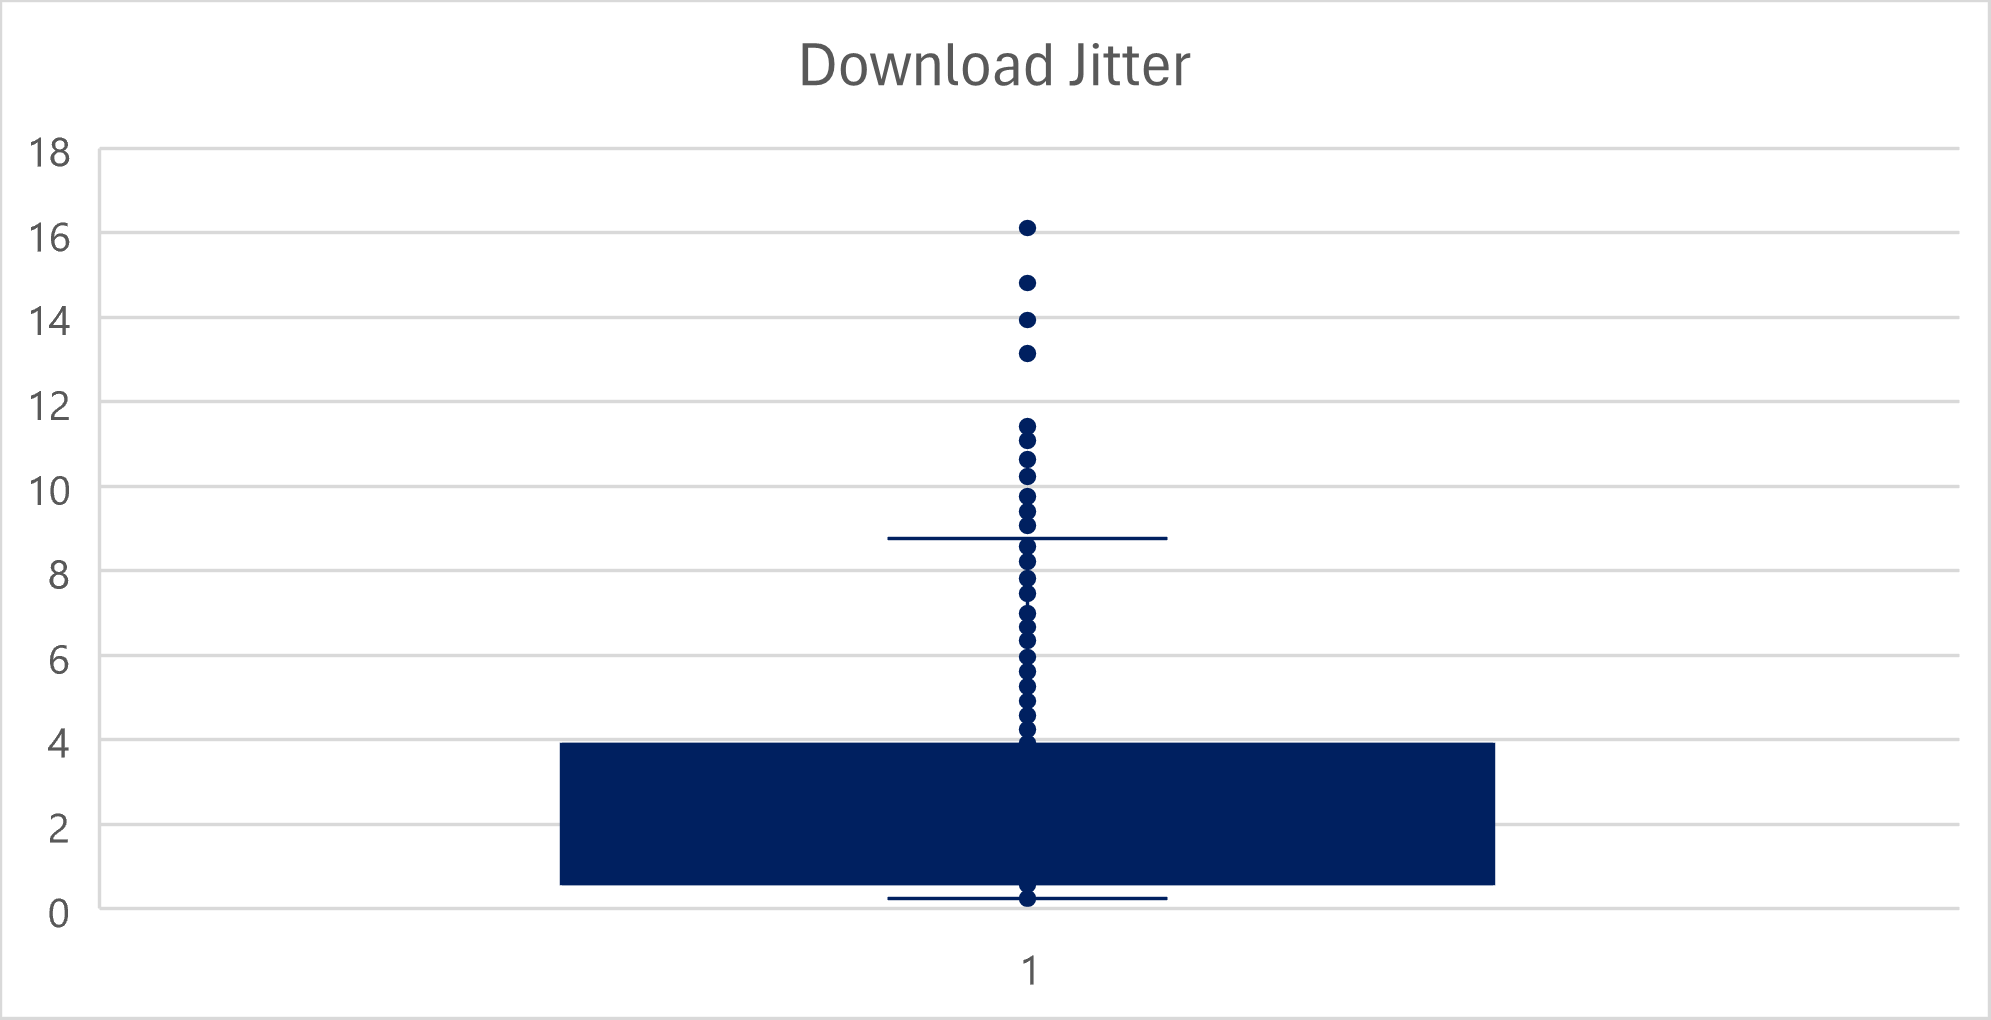
\includegraphics[width=8cm,height=6cm,keepaspectratio]{Figures/Picture3.png}}
    \caption{Class Interval for Download Speed.}
    \label{fig4}
\end{figure}

\begin{figure}[!htbp]
    \centerline{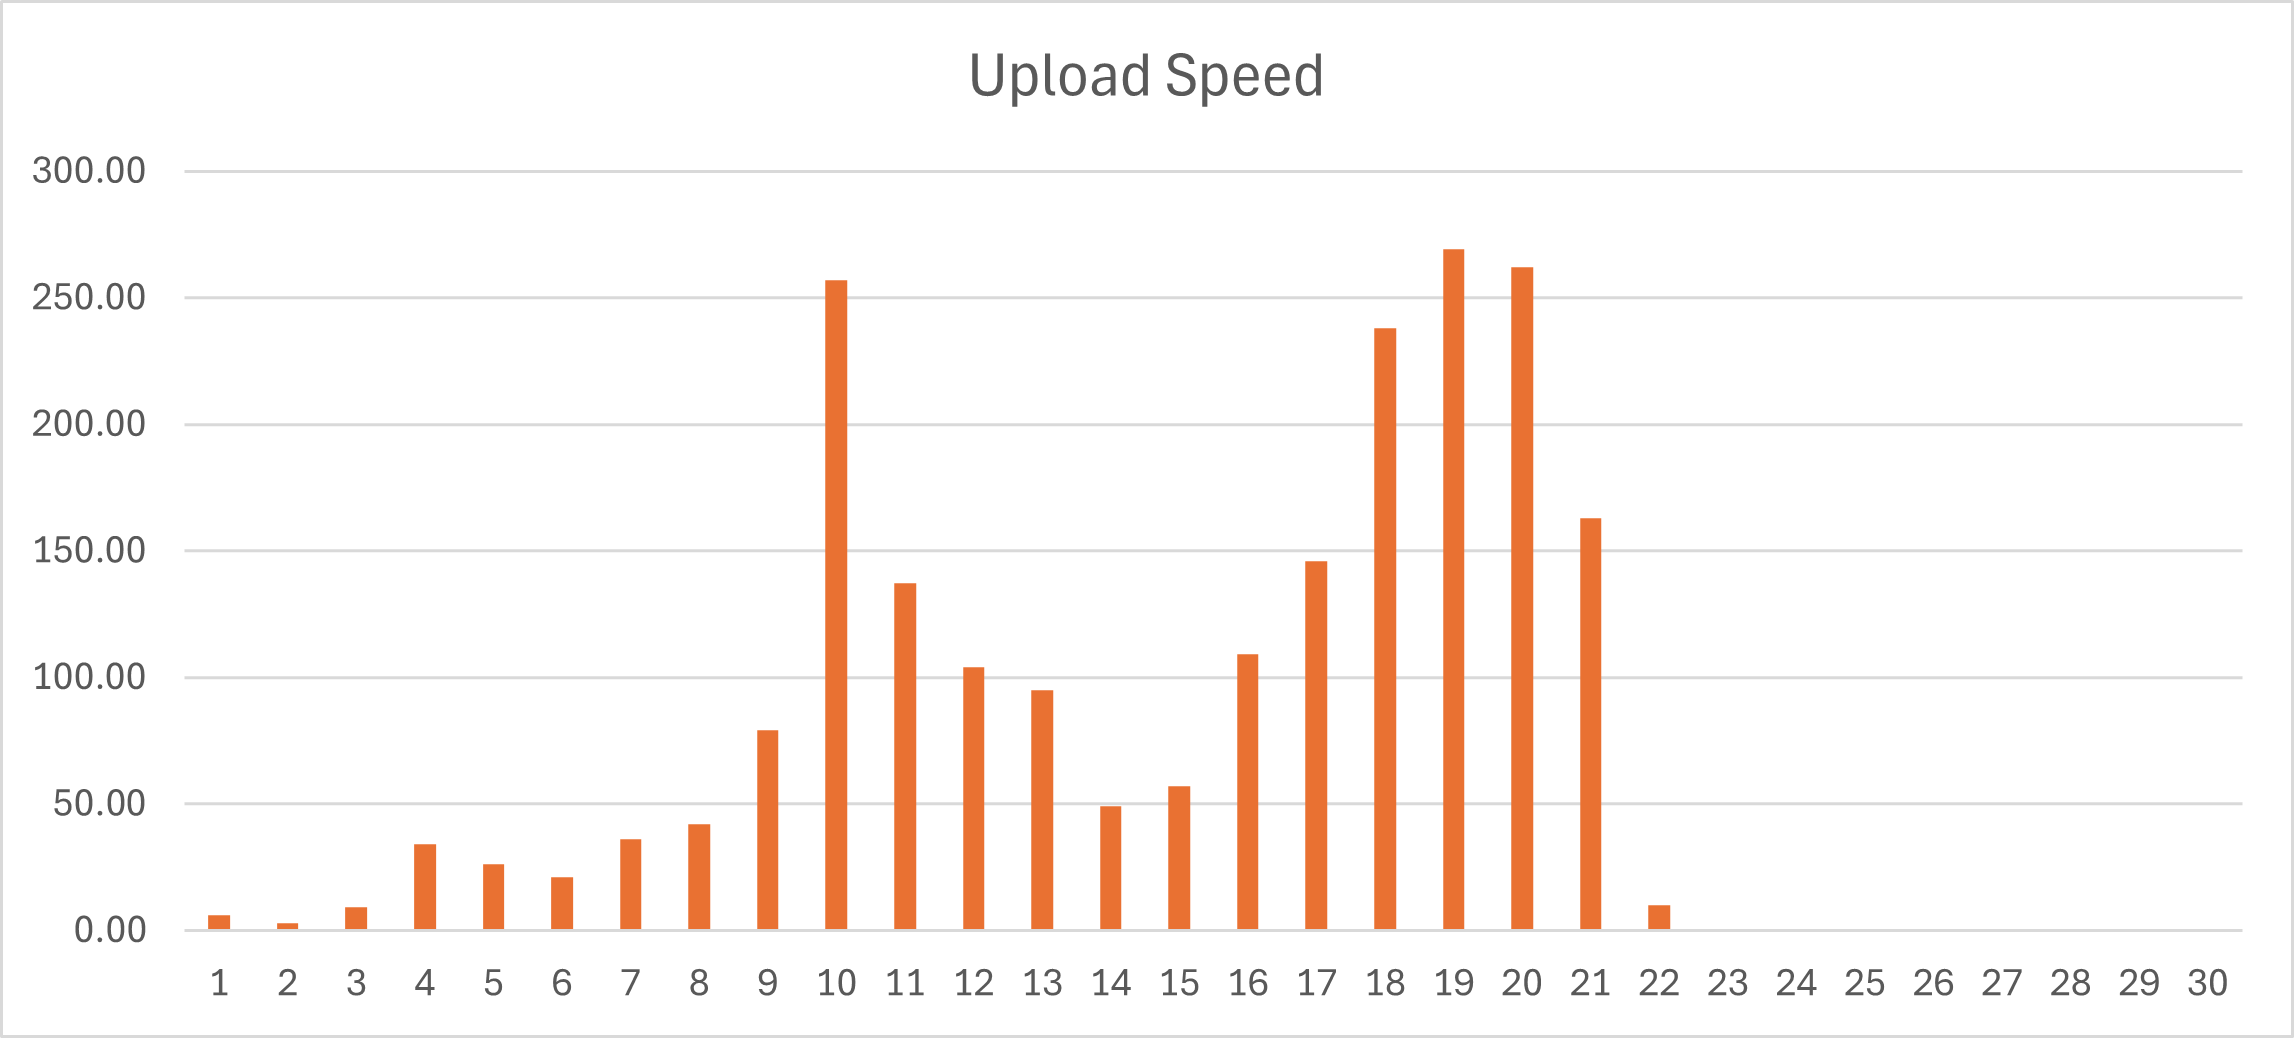
\includegraphics[width=8cm,height=6cm,keepaspectratio]{Figures/Picture4.png}}
    \caption{Class Interval for Upload Speed.}
    \label{fig5}
\end{figure}

\begin{figure}[!htbp]
    \centerline{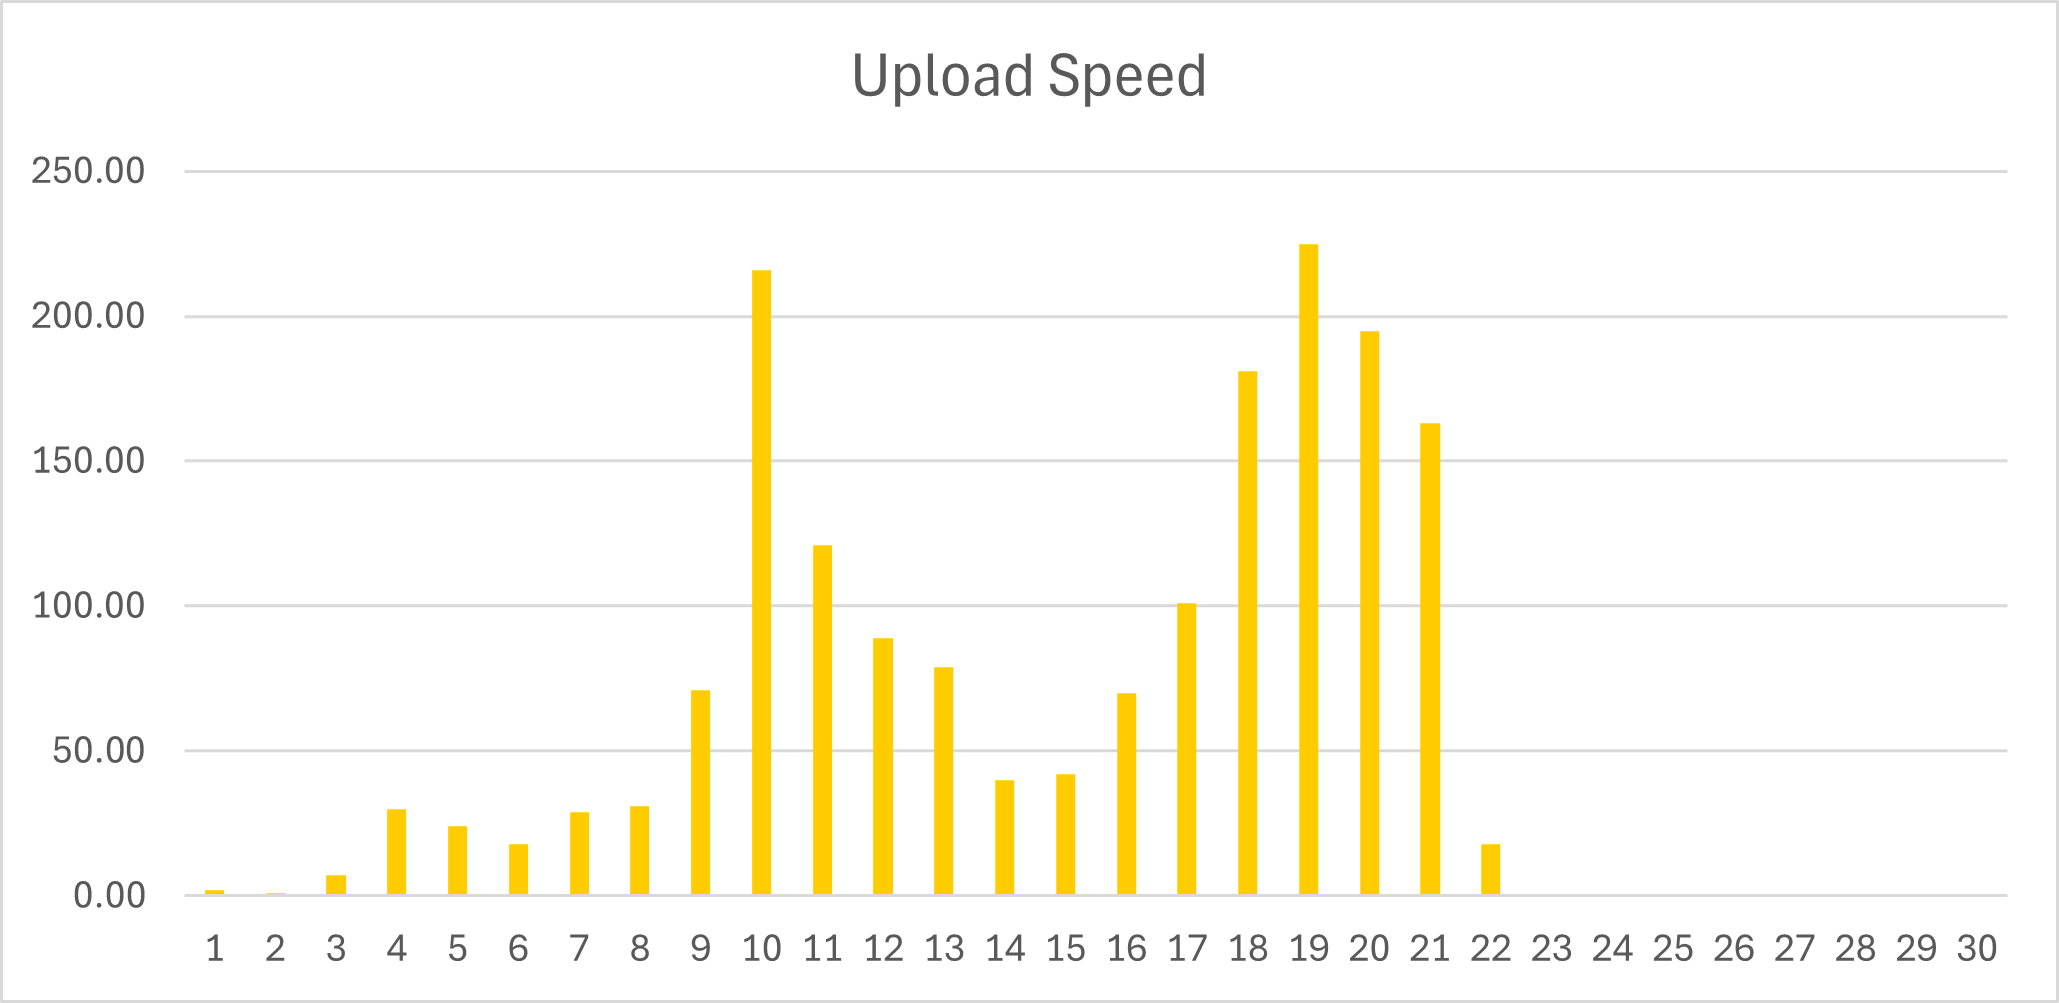
\includegraphics[width=8cm,height=6cm,keepaspectratio]{Figures/Picture5.png}}
    \caption{Class Interval for Ping.}
    \label{fig6}
\end{figure}

\begin{figure}[!htbp]
    \centerline{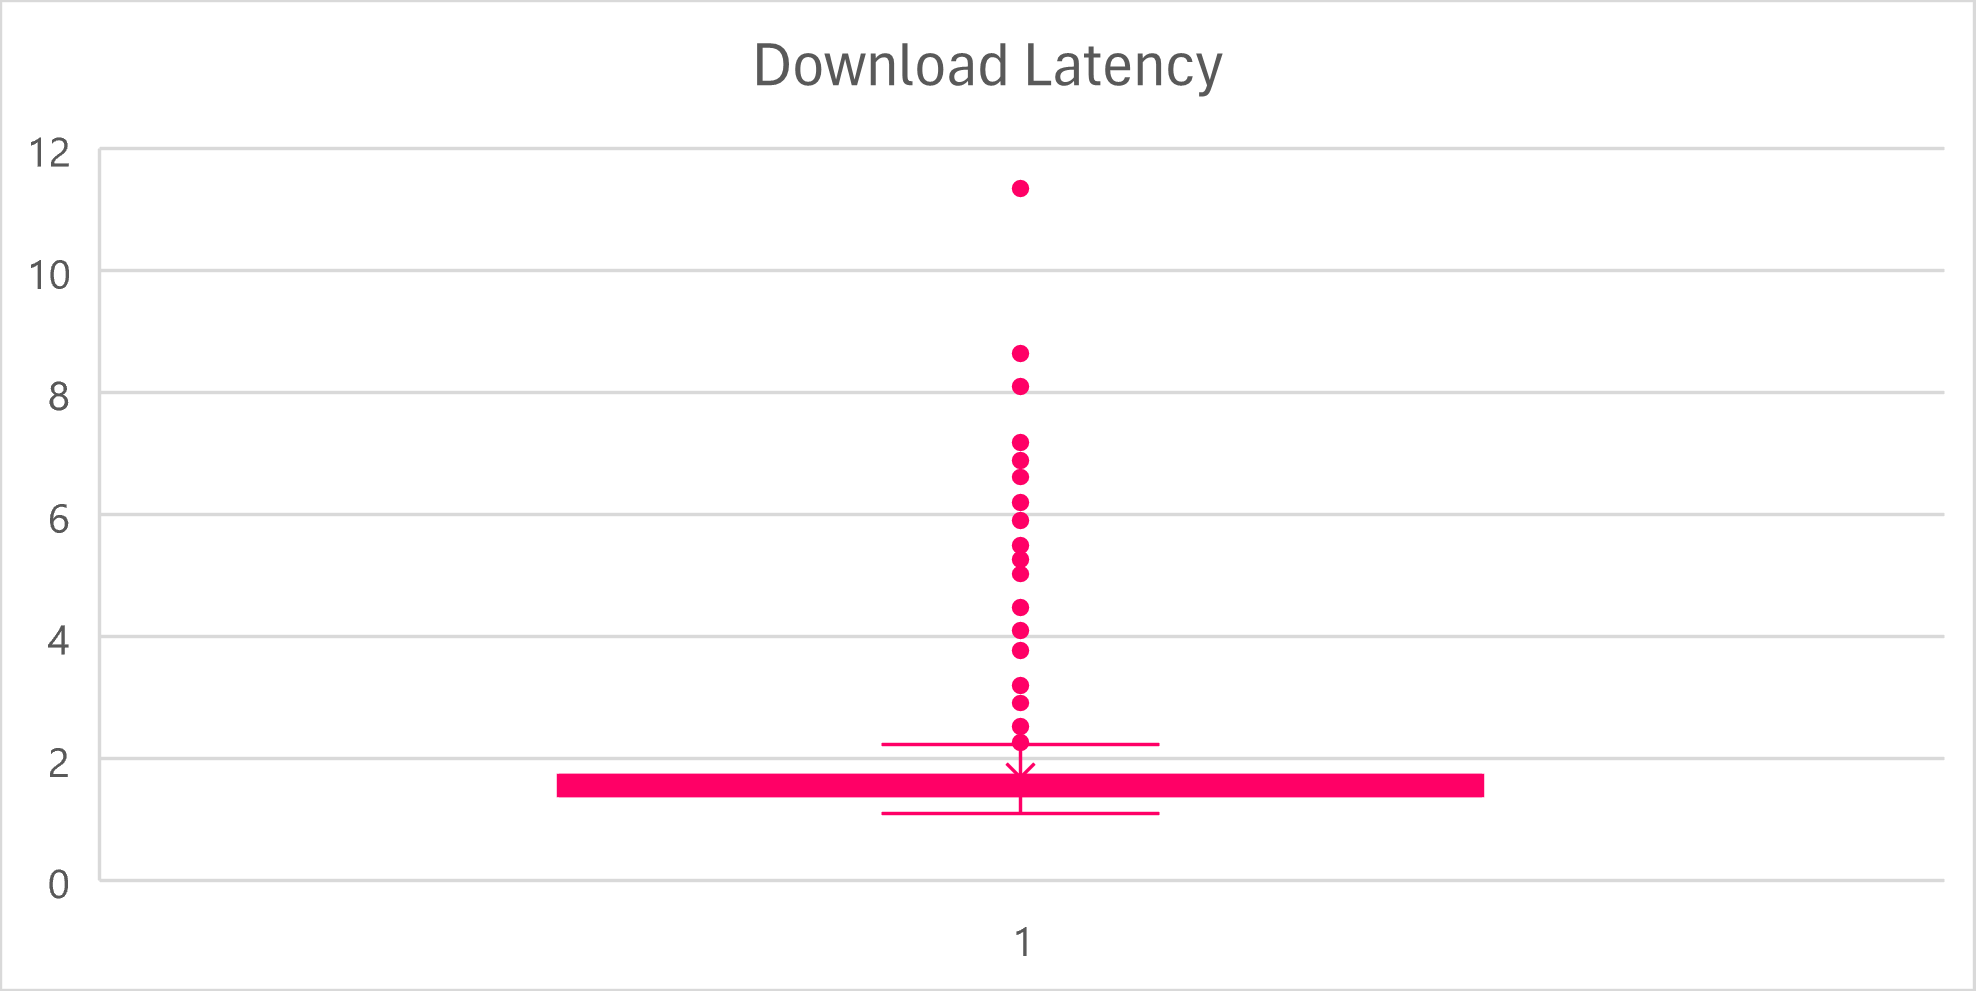
\includegraphics[width=8cm,height=6cm,keepaspectratio]{Figures/Picture7.png}}
    \caption{Time Series for Internet Speed.}
    \label{fig6}
\end{figure}

\begin{figure}[!htbp]
    \centerline{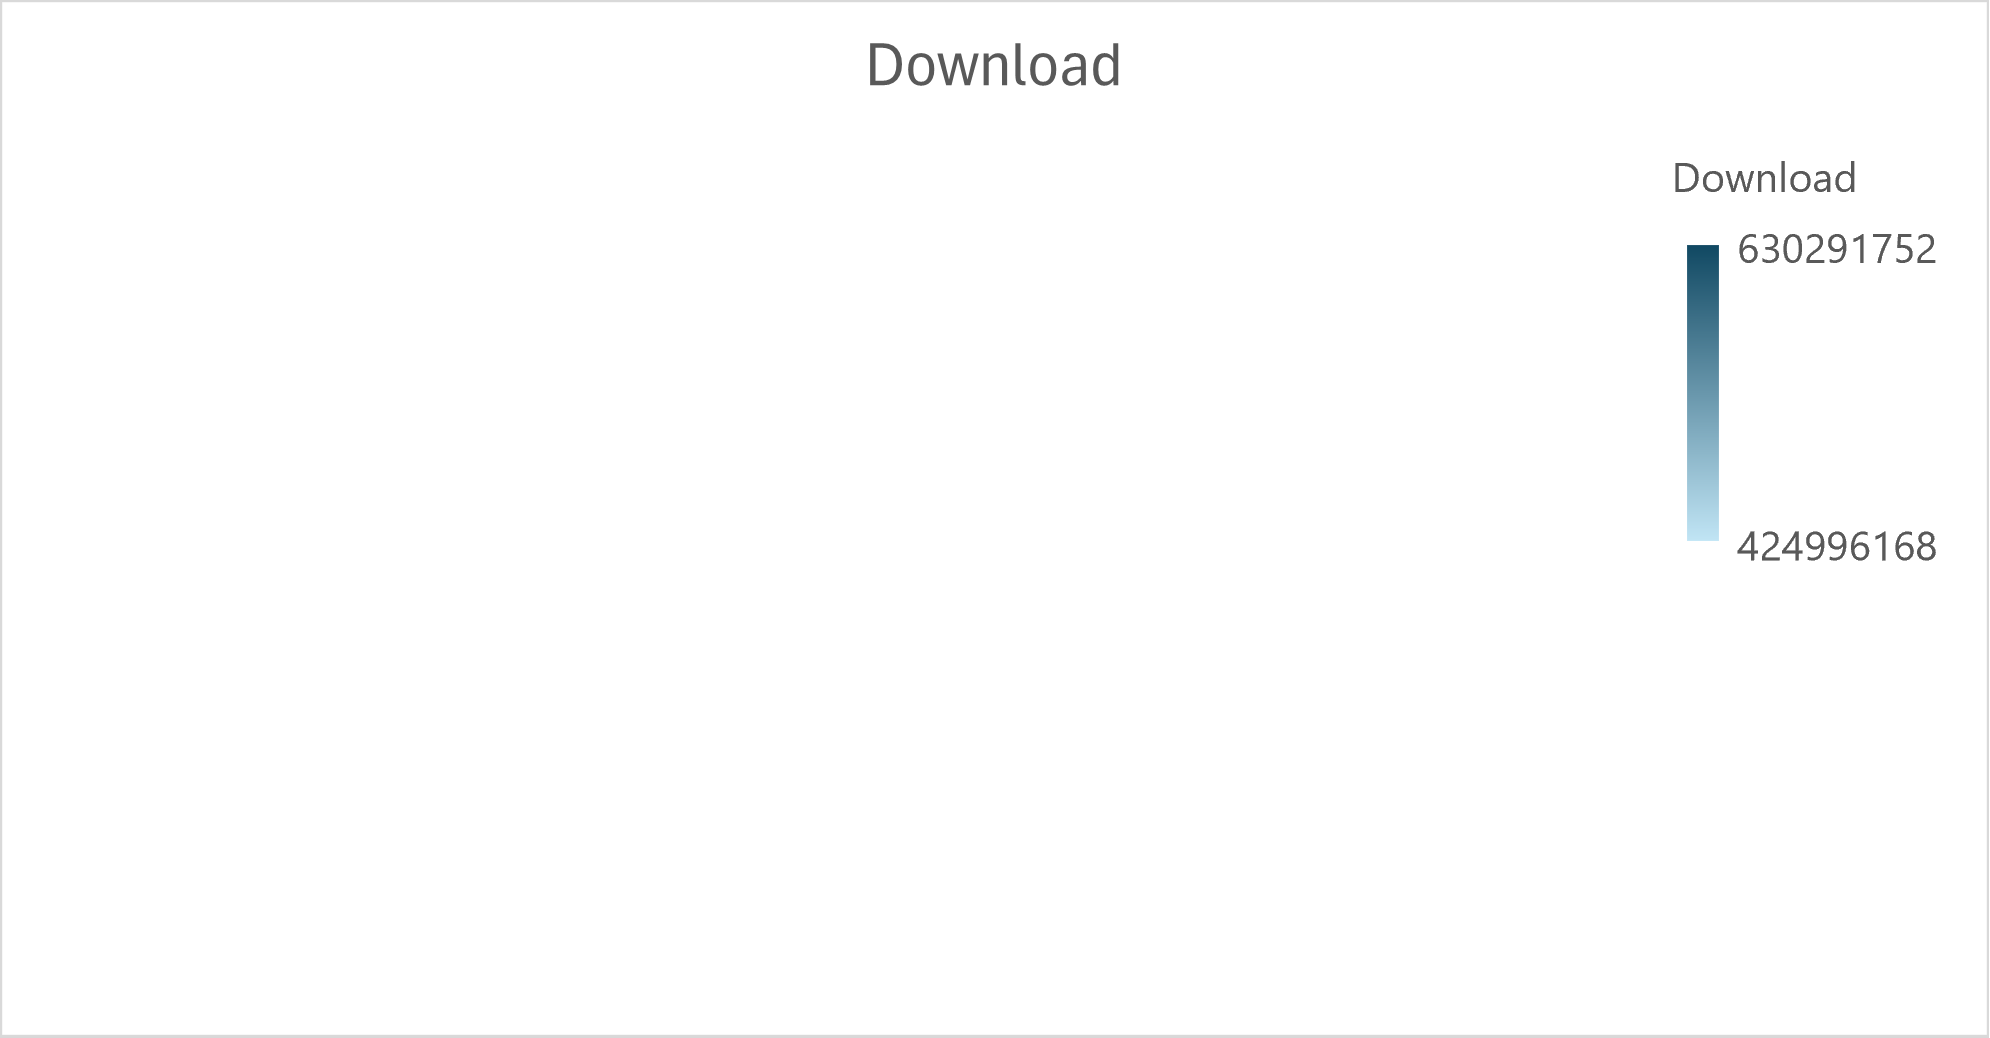
\includegraphics[width=8cm,height=6cm,keepaspectratio]{Figures/Picture8.png}}
    \caption{Time Series for Ping Jitter.}
    \label{fig6}
\end{figure}

\newpage

\section{Discussion}
This research was conducted within the span June 19, 2024 to July 10, 2024 and has 2149 datasets. If people would want to improve this data, future researchers should follow the same methodology of the experiment but increase the time at which they perform the experiment. A longer experiment will naturally provide more accurate results as this approach gives data that will be closer to the mode of internet performance metrics for a particular internet's all time performance. 
In this experiment, the researchers also only used PLDT as their ISP. The information on this paper suggests that monitoring the services of multiple ISPs will give different results per ISP. The organized sections of data from this experiment will allow its readers to compare data from different ISPs. Meanwhile, this gathered data could validate the feasibility of the methodology of this experiment if outliers exist within the data. 
The Internet exists for its practical usage, so it is suggested that future researchers test internet performance on multiple devices, but one at a time, and different softwares to analyze the performance of the internet with changing variables. This experiment aims to validate the performance of the internet through its ping, download, upload speeds, etc. for the reason of estimating its internet quality in practical use. With this information, it is suggested that future researchers evaluate the performance of the internet within the said parameters.
An important concern of the researchers of this study is that the current reviews for PLDT show itself as a completely different result from the data of this experiment. In the Philippines, PLDT is known to have one of the worst customer satisfaction due to its poor internet services and unsatisfactory customer service. However, this research indicates that the internet speed of PLDT may not exactly be of substandard quality. For this reason, the researchers recommend more tests on PLDT as an internet service provider (ISP) to question the preeminent perspective of Filipinos towards PLDT.

\section{Conclusion}
PLDT has proven itself as a reliable internet service provider (ISP) because the measurements of the internet data in the experiment exceed the agreed plan of the internet that was tested in this paper. 
The download and upload speed both exceed the internet plan of 600 mbps. This data shows that the null hypothesis was rejected as the performance of the internet exceeded its critical value of 600 mbps. 
For gamers who may find this information helpful, the speed of the tested PLDT internet in this experiment varies above 20\% from a ping of 1 milliseconds. 
In other words, this internet should be relatively good for online games.

\begin{thebibliography}{00}
\bibitem{b1} S. Bauer et al., “Understanding broadband speed measurements”, MIT. Accessed: June 30,2024. [Online]. Available: https://groups.csail.mit.edu/ana/Publications/Understanding\_broadband\_
speed\_measurements\_bauer\_clark\_lehr\_TPRC\_2010.pdf.
\bibitem{b2} S. Bebortta and S. K. Das, "Assessing the Impact of Network Performance on Popular E-Learning Applications," 2020 Sixth International Conference on e-Learning (econf), Sakheer, Bahrain, 2020, pp. 61-65, doi: 10.1109/econf51404.2020.9385497.
\bibitem{b3} A. Boonsongsrikul et al., "Performance Metrics and Strategy for Evaluating Internet Speed Tests in Fixed Broadband Networks," 2024 IEEE International Conference on Big Data and Smart Computing (BigComp), Bangkok, Thailand, 2024, pp. 424-428, doi: 10.1109/BigComp60711.2024.00093.
\bibitem{b4} X. Deng et al., “Comparing Broadband ISP Performance using Big Data from M-Lab”, arXiv, Jan. 24, 2021, doi: 10.48550/arXiv.2101.09795.
\bibitem{b5} R. B. Ikhsan et al., "Customer Loyalty Based On Internet Service Providers-Service Quality," 2022 6th International Conference on Informatics and Computational Sciences (ICICoS), Semarang, Indonesia, 2022, pp. 18-23, doi: 10.1109/ICICoS56336.2022.9930615.
\bibitem{b6} C. Overturf., “How does Speedtest measure my network speeds?” SPEEDTEST. Accessed: June 30, 2024. [Online]. Available: https://help.speedtest.net/hc/en-us/articles/360038679354-How-does-Speedtest-measure-my-network-speeds
\bibitem{b7} E. M. Rio, Jr.,  “rules and regulations implementing republic act (r.a.) no. 10929 known as the free internet access in public places act”. DICT. Accessed: June 30, 2024. [Online]. Available: https://dict.gov.ph/wp-content/uploads/2017/12/IRR-RA-10929-Version-8.pdf.
\bibitem{b8} A. Saengsai et al., "Broadband Internet Speed Dashboard for Sustainable Service Improvement in Thailand," 2024 IEEE International Conference on Big Data and Smart Computing (BigComp), Bangkok, Thailand, 2024, pp. 418-423, doi: 10.1109/BigComp60711.2024.00092. 
\bibitem{b9} R. Sharma et al., “Measuring the Prevalence of WiFi Bottlenecks in Home Access Networks,” arXiv, Nov. 9 2023, doi: 10.48550/arxiv.2311.05499.
\bibitem{b10} S. Hasan and W. Woo, “What's my Daily Value? Interpretation of network performance metrics in broadband consumer labels”, Association for Computing Machinery, New York, NY, USA, 2023, pp. 8-24, doi: 10.1145/3609396.3610546

\end{thebibliography}

\end{document}
